\documentclass[10pt]{article}

\usepackage[margin=1.5cm, includefoot, footskip=30pt]{geometry}

\usepackage{amssymb}
\usepackage{amsmath}
\usepackage{booktabs}
\usepackage{caption}
 \usepackage{epsfig}
\usepackage{graphicx}
\usepackage{hyperref}
\usepackage{psfrag}
\usepackage{subcaption}
\usepackage{ulem}
\usepackage{standalone}
\usepackage{tikz}

\newcommand{\rd}{\mathrm{d}}
\newcommand{\be}{\begin{eqnarray}}
\newcommand{\ee}{\end{eqnarray}}
\usepackage{tabularx} % http://ctan.org/pkg/tabularx
\renewcommand{\arraystretch}{1.5} % tables have longer cells

\newtheorem{theorem}{Theorem}

% \journal{Undecided Journal}

\title{An evolutionary game theory model for devaluing rhinos}
\author{Nikoleta E. Glynatsi, Vincent Knight, Tamsin E. Lee} %TODO Authors
\date{}

\begin{document}

\maketitle

\begin{abstract}

Rhino poaching has escalated in recent years due the demand for rhino horn in 
Asian countries. Rhino horn is used in Traditional Chinese Medicine and as a 
status symbol of success and wealth. Wild life managers attempt to minimise
the rhino casualties with approaches such as devaluation of the rhino horn. 
The  most common strategy of devaluing horns includes dehorning. In~\cite{Lee}
game theory modelling was used to examined the interaction of poachers and
wild life managers.  A manager can either `dehorn' their rhinos or leave the
horn attached. Poachers may chose to to behave `selectively' or `indiscriminately'.
The approach described in this paper builds upon~\cite{Lee} and investigates 
the interactions  between the poachers using evolutionary game theory. 
Evolutionary game theory, allows us to explore the evolutionary stabilities 
of the strategies available to a poacher. The purpose of this work is to discover
the conditions which best  encourages the poachers to behave selectively, that
is, they only kill those rhinos with full horns.  The results show that, poachers
will never chose to behave selectively as long as there is even the slightest
gain from a partial horn. Thus, we advice wild life managers to spend more of
the their resources into security and not in dehorning rhinos.
\end{abstract}

%=============================================
\section{Introduction}\label{section:introduction}

The illegal trade in rhino horn supports aggressive poaching syndicates and a 
black market (Nowell et al., 1992). This lucrative market entices people to invest
their time and energy to gain a `winfall' in the form of a rhino horn, through the 
poaching of rhinos. In recent years poaching has escalated to an unpresidented 
level resulting in concerns over their future existence (Smith et al., 2013). In 
response, rhino conservation has seen increased  ilitarisation with `boots on the 
ground' and `eyes in the sky' (Duffy et al., 2015). An alternative method is to 
devalue the horn itself, one of the main  methods being the removal so that only
a stub is left. The first attempt at large-scale rhino dehorning as an anti-poaching
measure was in Damordond,  Namibia, in 1989 (Milner-Gulland and Leader-Williams,
1992). Other methods of devaluing the horn that have been suggested include
the insertion of poisons, dyes or GPS trackers (Gill, 2010; Smith, 2013). However, 
like dehorning, they cannot remove all the potential gain from an intact horn 
(poison and dyes fade or GPS trackers can be removed). This paper builds on 
the work of \cite{Lee} and considers the general strategy of devaluing horns,
which includes dehorning.

Rhino populations now persist largely in protected areas or on private land, and
require intensive protection (Ferreira et al., 2014). For wildlife managers law 
enforcement is often one of the main methods of deterring poaching, however 
rhino managers can remove the poaching incentive by devaluing their rhinos 
(Milner-Gulland, 1999). Milner-Gulland and Leader-Williams (1992) found the 
optimum proportion to dehorn using mean horn length as a measure of the 
proportion of rhinos dehorned. They showed, with realistic parameter values, 
that the optimal strategy is to dehorn as many rhinos as possible. 
A manager does not need to choose between law enforcement or devaluing, but
perhaps adopt a combination of the two; especially given that devaluing rhinos 
comes at a cost to the manager, and the process comes with a risk to the rhinos.

A recent paper modelled the interaction between a rhino manager and poachers
using game theory~\cite{Lee}.  The authors consider a working year of a single 
rhino manager.  A manager is assumed to have standard yearly resources which
can be allocated on devaluing a proportion of their rhinos or spent on security. 
It is assumed that all rhinos initially have intact horns. Poachers may either only
kill rhinos with full horns, `selective poachers', or kill all rhinos they encounter, 
`indiscriminate poachers'. If all rhinos are left by the rhino manager with their 
intact horns, it does not pay poachers to be selective so they will chose to be 
indiscriminate. Conversely, if all poachers are selective, it pays rhino managers 
to invest in devaluing their rhinos. This dynamic is represented in Fig.~\ref{fig:RhinoPic}.
Assuming poachers and managers will always behave so as to maximise their 
payoff, there are two equilibriums: either all devalued and all poachers selective;
or all horns intact and all poachers indiscriminate. Essentially, either the managers 
win, the top left quadrant of Fig.~\ref{fig:RhinoPic}, or the poachers win, the bottom
right quadrant of Fig.~\ref{fig:RhinoPic}. The paper concludes that poachers will
always choose to behave indiscriminately, and thus the game settles to the top
left quadrant, i.e., the poachers win.

\begin{figure}[!htbp]
	\centering
	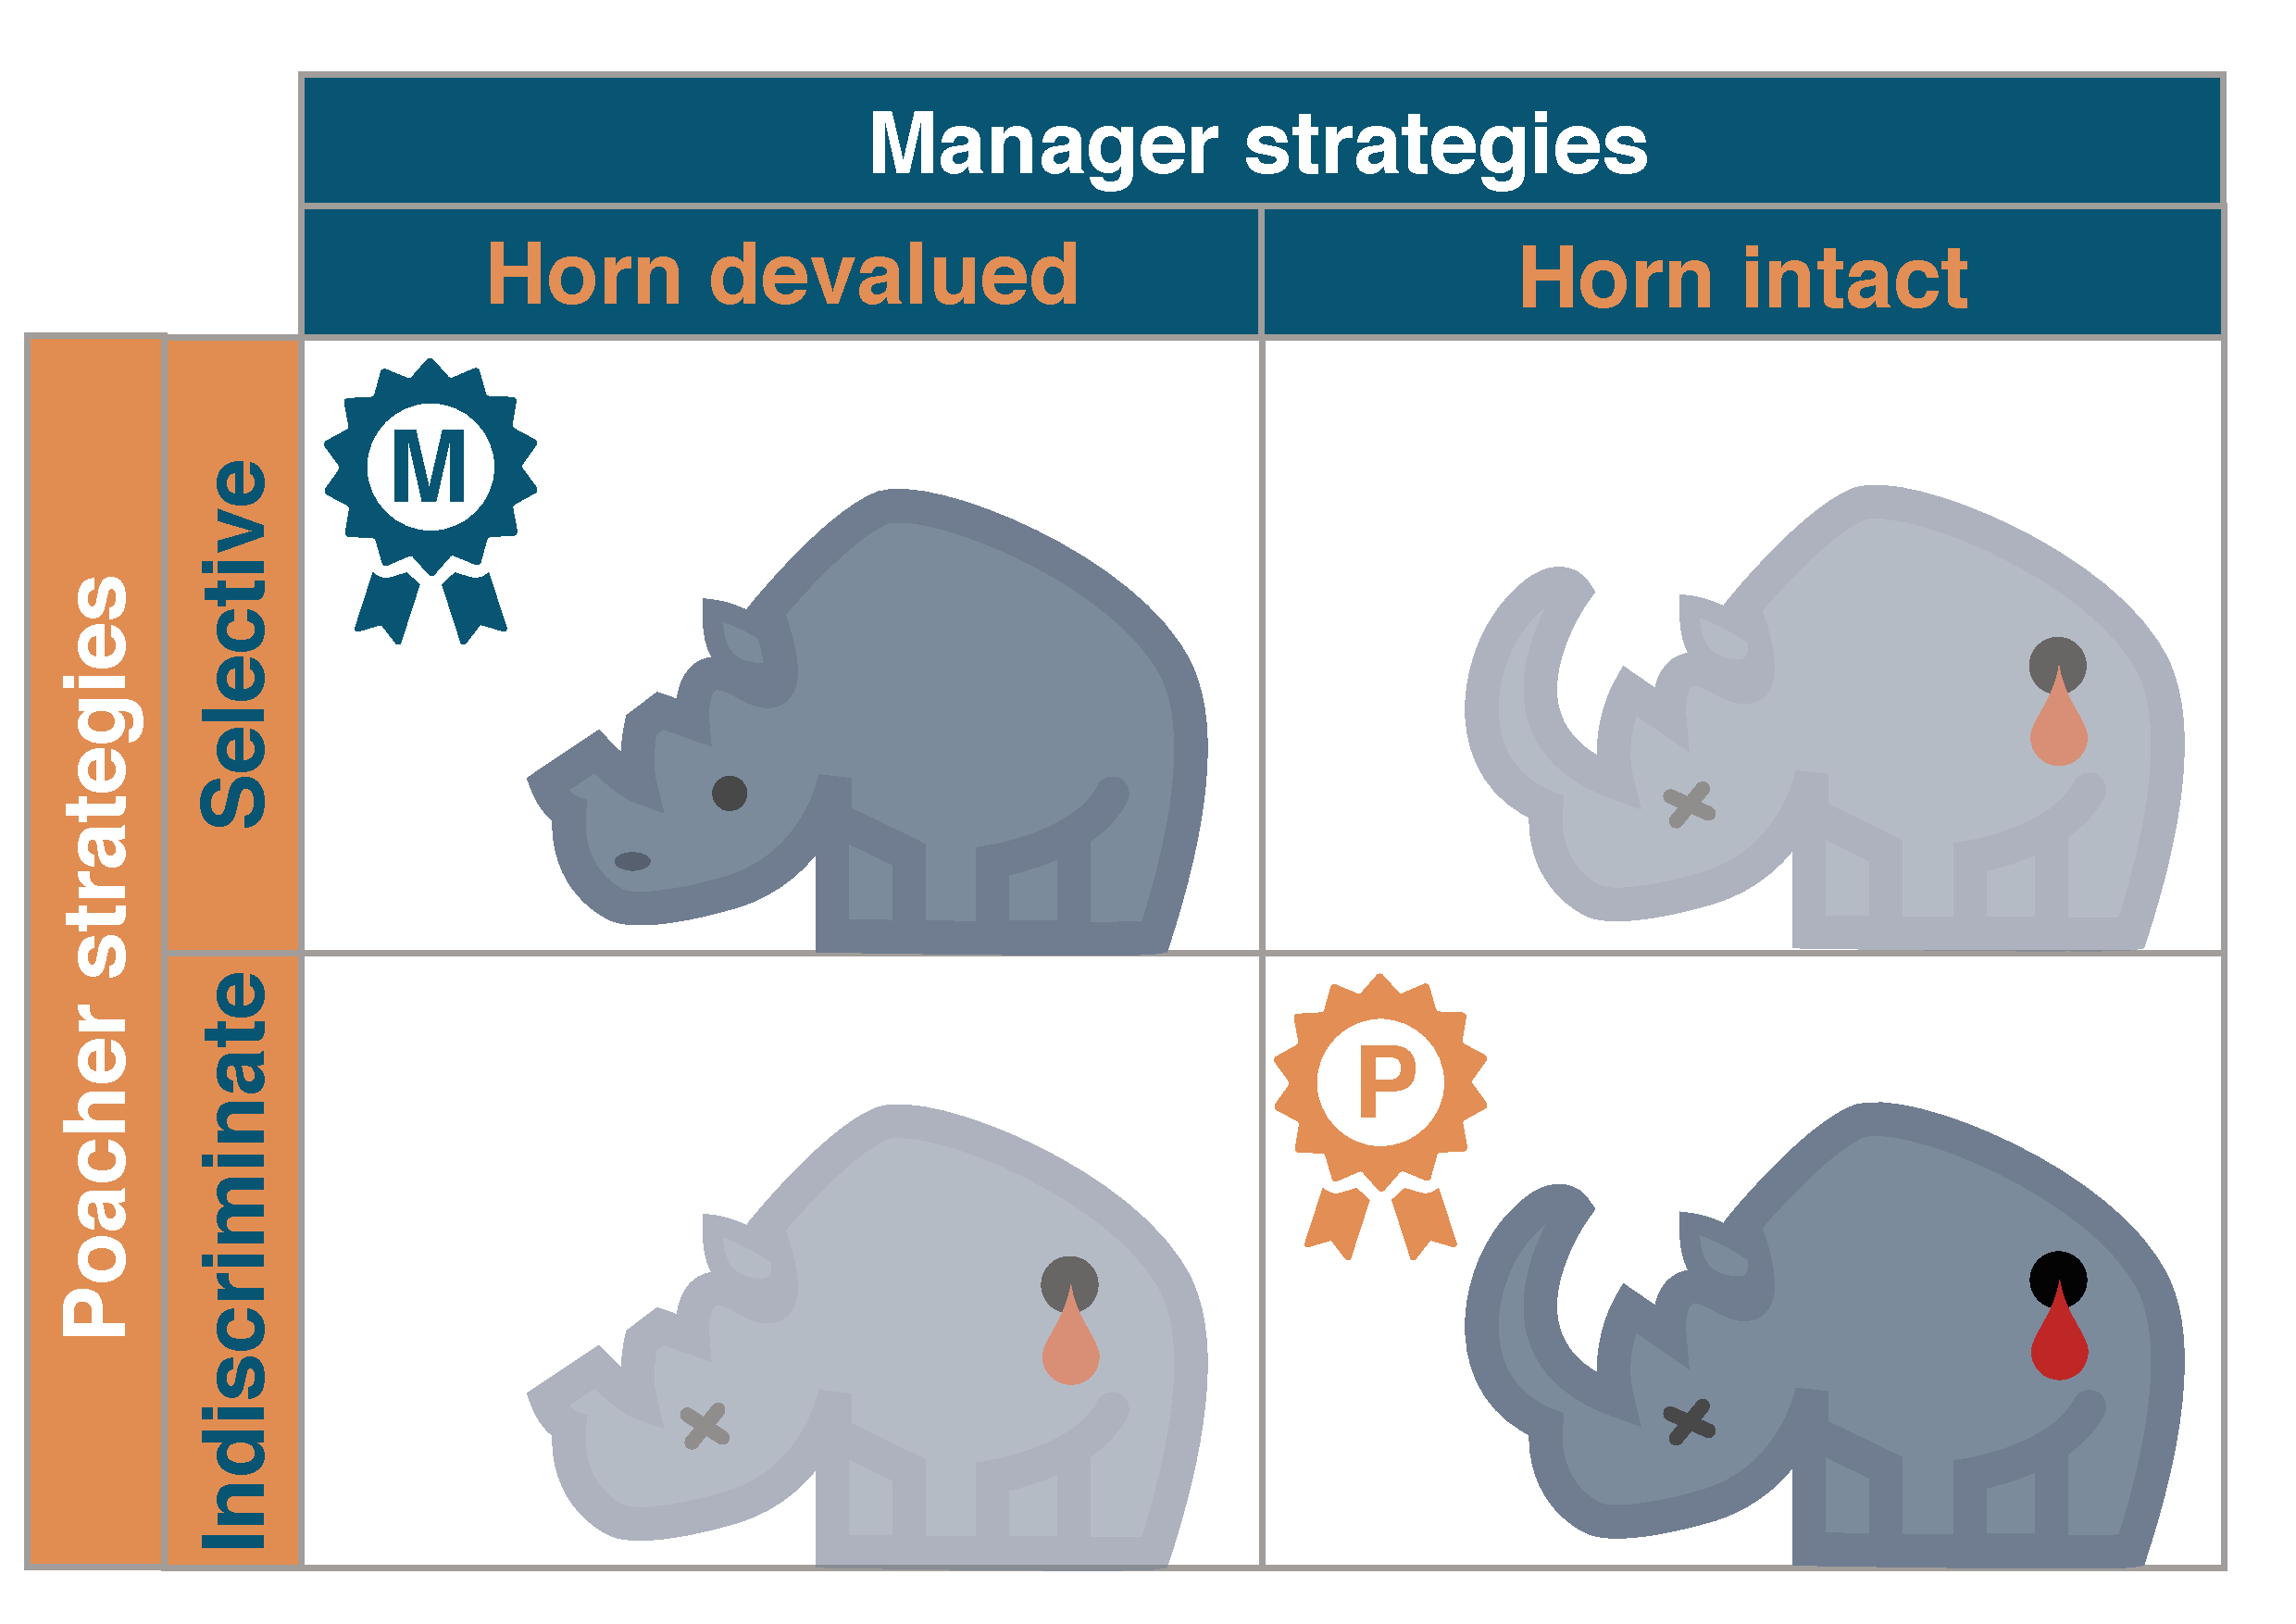
\includegraphics[scale=0.2]{images/RhinoPic.pdf}
	\caption{\label{fig:RhinoPic} The game between rhino manager and rhino 
	poachers. The system settles to one of two equilibriums, either devaluing is effective or not.}
\end{figure}

The work of~\cite{Lee} did not take in to account the population dynamic effect
of  these strategies. In a population full of selective poachers would their be 
a benefit to a single poacher becoming indiscriminate or vice versa? This notion 
is explored here using evolutionary game theory~\cite{Smith}. The 
game is not that of two players anymore (manager and poacher) but an infinite
population of poachers is considered. This allows for interaction between poachers
over multiple plays of the game to be explored with the rhino manager being the
one that creates the conditions of the population. 

In evolutionary game theory, we assume infinite populations and in our
model this will be represented by \(\chi=(x_1, x_2)\) with \(x_1\) proportion of the
population using a strategy of the first type and \(x_2\) of the second, denoted
by \(s_1, s_2\) respectively. We assume there is a utility function \(u_1\) and 
\(u_2\) that maps the population to a fitness for each type,

\[ u_1(\chi)  \qquad u_2(\chi).\] 

In evolutionary game theory these utilities are used to dictate the evolution of
the population over time, according to the following differential equations,

\begin{eqnarray}
	\label{eqn:u_differential_eq}
	\left\{
	\begin{array}{cl}
	\dfrac{dx_1}{dt}=x_1(u_1(\chi)-\phi),
	\\
	\\
	\dfrac{dx_2}{dt}= x_2(u_2(\chi)-\phi).
	\end{array} \right.
\end{eqnarray}

The overall population is assumed to remain stable thus, \(x_1 + x_2 = 1 \)
and

\begin{eqnarray}
	\dfrac{dx_1}{dt}  + \dfrac{dx_2}{dt} = 0 \Rightarrow x_1(u_1(\chi) - \phi)
	 + x_2(u_2(\chi) - \phi)=0.
\end{eqnarray} 

As follows the average fitness can be written as,

\begin{eqnarray}
\label{eqn:average_fitness}
	\phi=x_1u_1(\chi) + x_2u_2(\chi).
\end{eqnarray}

By substituting (\ref{eqn:average_fitness}) and \(x_2= 1 - x_1\) in (\ref{eqn:u_differential_eq}),

\begin{eqnarray}
	\label{eqn:u_differential_simplified}
	\frac{dx_1}{dt}= x_1(1 - x_1)(u_1(\chi) - u_2(\chi)).
\end{eqnarray}

The equilibria of the differential equation (\ref{eqn:u_differential_simplified})
are given by,

\begin{itemize}
	\item \(x_1=0\),
	\item \(x_1=1\),
	\item \(x_1 \in (0, 1) \mbox{ for } u_1(\chi)=u_2(\chi)\).
\end{itemize}

Thereupon, two notions must be checked for the equilibria,

\begin{itemize}
	\item stability. The notion of stability implies that the underlying differential
	equation does not move. A strategy is the best response in the population
	that it generated. Secondly, 
	\item evolutionary stability. The notion of evolutionary stability implies
	that the  differential equation ...
\end{itemize}

The notion of evolutionary stability can be checked only for the stable strategies.
For a stable strategy to be an evolutionary stable strategy (ESS) it must remain 
the best response even an mutated population \(\chi_\epsilon\). A mutated population is the post entry population, 
where a small proportion \(\epsilon\) starts deviating and adopts a different strategy.
The mutated population can be thought as a nudged.  Assume Fig.
\ref{fig:stable_ess_driagrams}, is illustrating two stable strategies. In Fig.
\ref{fig:stable_diagram}, though the population has reached a stable point once 
a nudge is applied the marble will lose it's position. In contrast, Fig.~\ref{fig:ess_diagram}
illustrates a strategy that even when nudged the marble will bounce back to it's
original position, making it ESS.

\begin{figure}[!htbp]
\begin{center}
    \begin{subfigure}{0.40\textwidth}
	\includestandalone[width =\textwidth]{images/stable}
	\caption{\label{fig:stable_diagram} A diagram of a stable strategy which 
	is not ESS.}
    \end{subfigure}
    \begin{subfigure}{0.40\textwidth}
	\includestandalone[width = \textwidth]{images/evolutionary_stability}
	\caption{\label{fig:ess_diagram}A diagram of a stable strategy which is ESS.}
    \end{subfigure}
    	\caption{\label{fig:stable_ess_driagrams} Diagrams of stable strategies.}
\end{center}
\end{figure}

In the following section~\ref{section:the_model}, we determine expressions
for \(u_1, u_2\) that correspond to a population of wild rhino poachers and we
explore the stability of the equilibria identified in~\cite{Lee}. The results
contained in this paper are proven analytically, and more specifically it is 
shown that,

\begin{itemize}
	\item all poachers behaving selectively is not a stable strategy,  
	\item a mixed population where selective and indiscriminate poachers
	learn to co exist can not hold and
	\item finally all poachers adopting a indiscriminate strategy was proven to
	be stable and an evolutionary stable strategy.
\end{itemize}
%============================================================
\section{The Model}\label{section:the_model}

A wild rhino poacher can adopt two strategies, to either behave selectively
or indiscriminately. Calculating the utility for each strategy the gain and cost
that poachers are exposed to must be taken into account. The poacher incurs a
loss from seeking a rhino, and the risk involved. The gain depends upon the value
of horn, the proportion of horn remaining after the manager has devalued the 
rhino horn and the number of rhinos (devalued and not).

Let us first consider the gain to the poacher, where \(\theta\) is the amount of 
horn taken. We assume rhino horn value is determined by weight only, a 
reasonable assumption as rhino horn is sold in a grounded form~\cite{Saverhino}.
Referring to Fig.~\ref{fig:RhinoPic}, clearly if the horn is intact, the amount of
horn gained is \(\theta=1\) for both the selective and the indiscriminate poacher.
If the rhino horn has been devalued, and the poacher is selective, the amount of horn 
gained is \(\theta=0\) as the poacher does not kill. However, if the poacher is 
behaving indiscriminately, the amount of horn gained is \(\theta = \theta_r\)
(for some \(0<\theta_r<1\)). 
Therefore, the amount of horn gained in the general case is

\begin{eqnarray}
	\label{eqn:theta}
	\theta(r, s) = s (1 - r) + (1 - s) ((\theta_r - 1) r + 1),
\end{eqnarray}

where \(r\) is the proportion of rhinos that have been devalued, and \(s\) is the 
proportion of selective poachers. Note that since \(\theta_r, r, s  \in [0, 1]\), then
\(\theta(r, s) > 0\). Standard supply and demand arguments imply that the value
of rhino horn decreases as the quantity of horn increases. Thus at any given time
the expected gain for a poacher is

\begin{eqnarray}
	\label{eqn:individual_gain}
 	H \theta(r,s)^{-\alpha},
\end{eqnarray}

where \(H\) is a scaling factor associated with the value of a full horn, and 
\(\alpha \geq 0\) is a constant that determines the precise relationship between
the quantity and value of the horn.  Fig.~\ref{fig:GainCurve}, verifies that the 
gain curve corresponds to a demand curve.

\begin{figure}[!htbp]
\centering
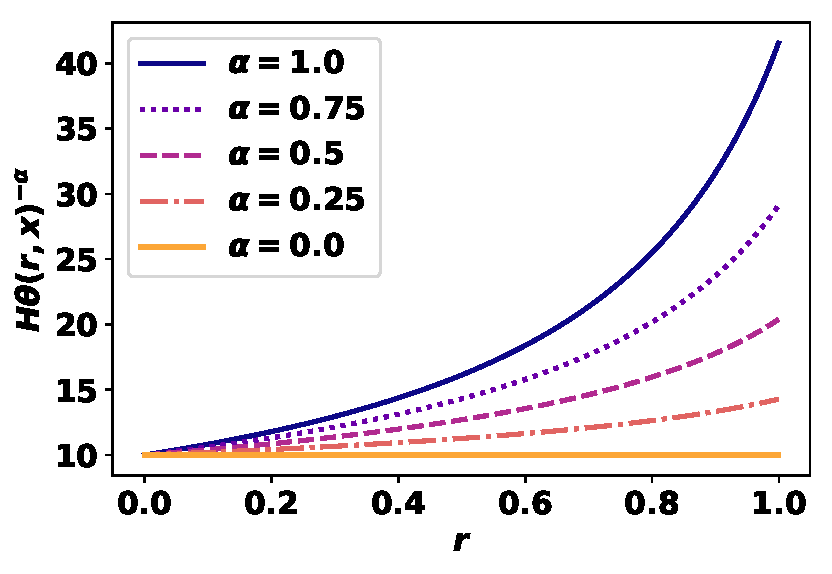
\includegraphics[width=0.4\textwidth]{images/gain_curve.pdf}
\caption{\label{fig:GainCurve} \(H \theta(r, s) ^{- \alpha}\) for values 
\(H = 10, \theta_r = 0.3\) and \(s = 0.2.\).}
\end{figure}

An individual interacts with the population, denoted as \(\chi=(x, 1 -x )\). Thus,
the gain is either

\begin{eqnarray}
	\label{eqn:gain}
	\left\{
	\begin{array}{cl}
	\theta(r, 1) H \theta(r, x)^{-\alpha} & \mbox{ selective poacher}
	\\
	\theta(r, 0) H \theta(r, x)^{-\alpha} & \mbox{ indiscriminate poacher}
	\end{array} \right.
\end{eqnarray}

depending on the chosen strategy of the individual, see Fig.~\ref{fig:RhinoPic}.
\\
\\
Secondly we consider the costs incurred by the poacher. Let us denote the number
of rhinos that will be considered at risk given \(r\) and \(s\) as \(\phi(r,s)\).
The rhinos \textbf{not} at risk are the devalued ones 
that cross the paths of selective poachers. Thus:

\begin{eqnarray}
	\label{eqn:psi}
	\psi(r, s) = 1 - rs.
\end{eqnarray}

Additionally, the poachers are also exposed to a risk. The risk to the poacher is
the opposite of the proportion of rhinos devalued \(r\), since the rhino manager
can spend more on security if the cost of devaluing is low.

\begin{eqnarray}
	\label{eqn:risk}
	(1 - r)^{\beta},
\end{eqnarray}

where \(\beta \geq 0\) is a constant that determines the precise relationship between
the proportion of rhinos not devalued and the security on the grounds. Therefore,
at any given time the expected cost for a poacher is, 

\begin{eqnarray}
	\label{eqn:individual_cost}
	\begin{array}{l}
	F \psi(r, s)^{\gamma} (1 - r)^{\beta} = F (1 - rs) ^{\gamma} (1 - r) ^{\beta}
	\end{array}
\end{eqnarray}

where \(F\) and \(\gamma \geq 0\) are constants that determine the precise relationship
between the proportion of vulnerable rhinos and the probability of finding a rhino,
such that \(\gamma\) close to zero indicates very sparse rhinos. Fig.
\ref{fig:CostCurves},  verifies the decreasing relationship between \(r\) and the
cost.

\begin{figure}[!htbp]
\begin{center}
    \begin{subfigure}{0.40\textwidth}
        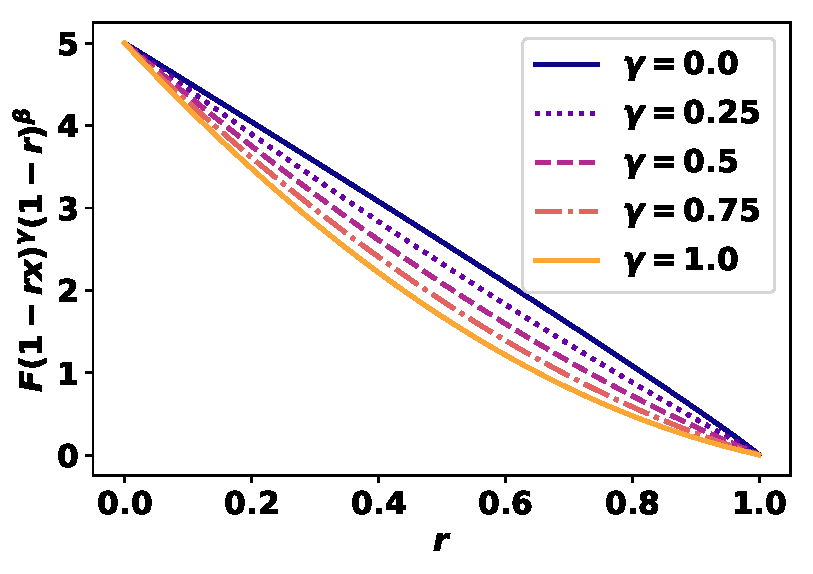
\includegraphics[width=\linewidth]{images/gammas_curve.pdf}
        \caption{For values, \(s=0.7, F=5\) and \(\beta=0.95\).}
    \end{subfigure}
    \begin{subfigure}{0.40\textwidth}
        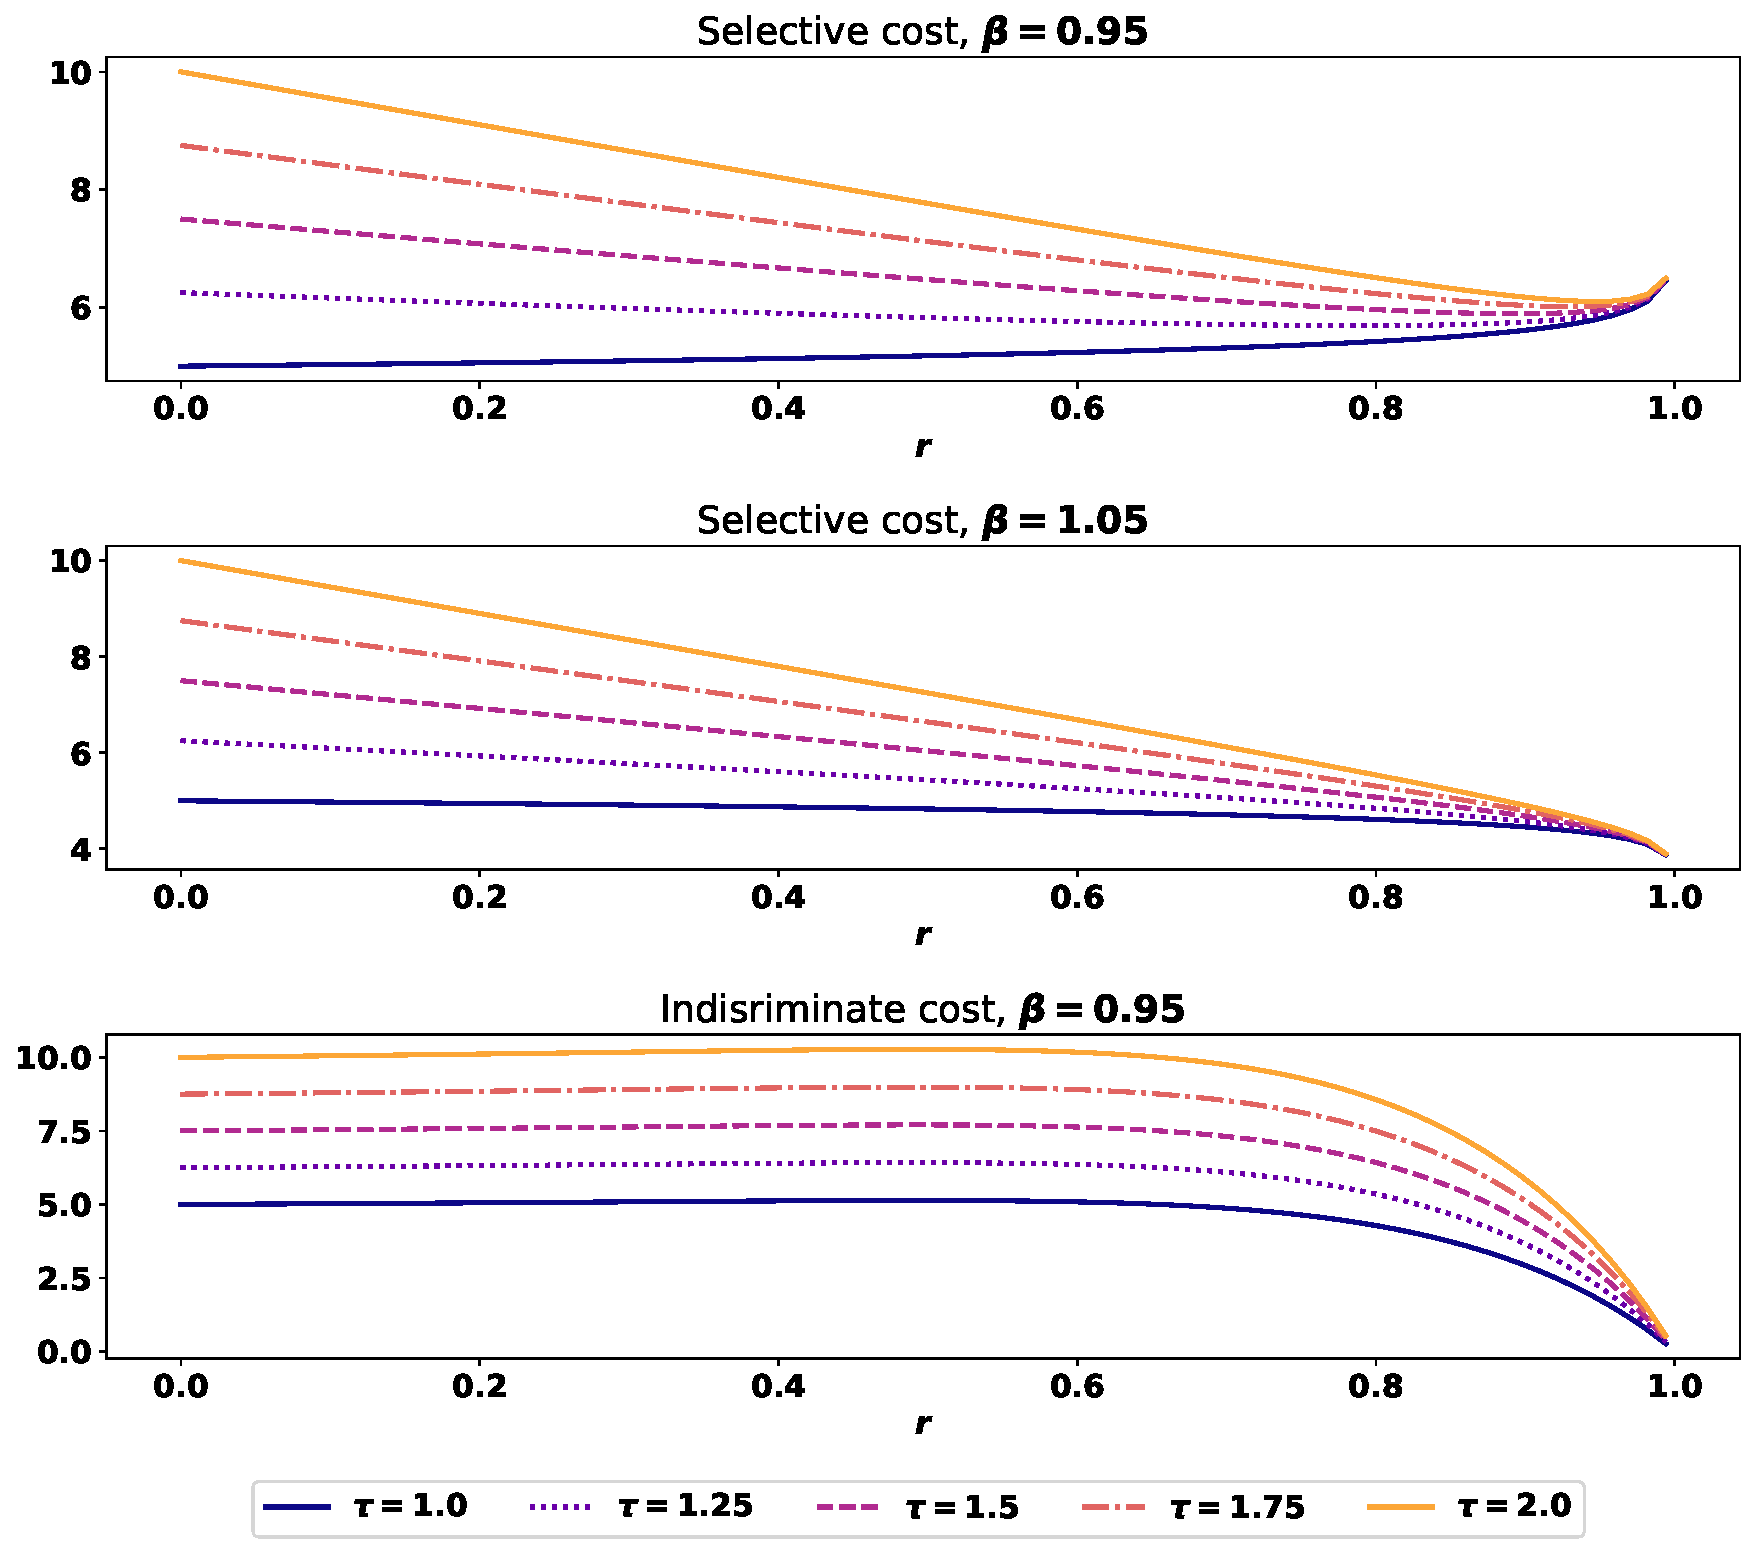
\includegraphics[width=\linewidth]{images/betas_curve.pdf}
        \caption{For values, \(s=1, F=5\) and \(\gamma=0.95\).}
    \end{subfigure}
\caption{\(F (1 - rs)^{\gamma} (1 - r)^{\beta}\).}\label{fig:CostCurves}
\end{center}
\end{figure}

Note that for a indiscriminate poachers \(s = 0\) the seeking 
cost (\ref{eqn:risk}) will always be \(1\), thus the cost of finding a rhino is greater
than the same cost for a selective poacher. However, a selective poacher needs 
more time to secure an `available' rhino, if they exist at all. Hence, an 
additional cost that tends to infinity as \(r \rightarrow 1\) must be applied, 

\begin{eqnarray}
	\label{eqn:selective_cost}
	\left\{
	\begin{array}{cl}
	\frac{1}{\psi(r, 1)} = \frac{1}{1 - r} & \mbox{ selective poacher}
	\\
	\frac{1}{\psi(r, 0)} = 1 & \mbox{ indiscriminate poacher}
	\end{array} \right.
\end{eqnarray}

To summarise, the cost incurred by a given individual when interacting with
the population is given by 

\begin{eqnarray}
	\label{eqn:cost}
	\left\{
	\begin{array}{cl}
	\frac{1}{1 - r}  F(1- rx)^{\gamma} (1-r)^{\beta}& \mbox{ selective poacher}
	\\
	F(1 - rx)^{\gamma} (1-r)^{\beta}& \mbox{ indiscriminate poacher}
	\end{array} \right.
\end{eqnarray}

As a result, the utility of the poachers can now be defined. Let \(\sigma = (s, 1 - s)\)
denote the strategy of an individual. Thus \(\sigma = (1, 0)\) represent an
individual poacher who is selective and \(\sigma = (0, 1)\) represent an individual
poacher who is indiscriminate. Combining~(\ref{eqn:gain}) and (\ref{eqn:cost})
gives the utility function for the individual poacher \(\sigma\) in the population
\(\chi\),

\begin{eqnarray}
\label{eqn:utility}
u(\sigma, \chi) = s u_1(\chi) +(1 - s) u_2(\chi),
\end{eqnarray}
where

\begin{eqnarray}
\label{eqn:USchi}
u_1(\chi) &=& \theta(r,1) H \theta(r,x)^{-\alpha}
- \frac{1}{1- r} F\psi(r, x)^{\gamma} (1-r)^{\beta} ,
\\
\label{eqn:UnotSchi}
u_2(\chi) &=& \theta(r,0) H \theta(r,x)^{-\alpha}
- F\psi(r, x)^{\gamma}  (1-r)^{\beta}.
\end{eqnarray}
Substituting~(\ref{eqn:USchi}) and~(\ref{eqn:UnotSchi}) into~(\ref{eqn:utility}) gives

\begin{eqnarray}
\label{eqn:tutility2}
u(\sigma, \chi) &=&
H (\theta_r r(1-s) - r + 1)\theta(r,x)^{-\alpha} - F\left(1-s + \frac{s}{1-r} \right)(1-rx)^{\gamma}(1-r)^{\beta} .
\end{eqnarray}

In section~\ref{section:evolutionary_stability}, the notions of stability
and evolutionary stability of these two strategies as well as a potential 
mixed strategy will be investigated.

%=======================================================
\section{Evolutionary Stability}\label{section:evolutionary_stability}

Using an evolutionary model to study the devaluation of wild rhinos allows us 
to gain insight on the evolutionary stability of the strategies and their conditions.
By definition, for a strategy to be an ESS it must first be stable.
In our model there are three possible stable distributions based on the
equilibria of equation (\ref{eqn:u_differential_simplified}),

\begin{itemize} 
	\item All poachers are selective \(s=1\);
	\item All poachers are indiscriminate \(s=0\);
	\item Mixed population of selective and indiscriminate poachers.
\end{itemize}

Each of the equilibria is being examined is the following subsections.

\subsubsection{All poachers are selective \(s=1\)}

All \textbf{selective}, \(\sigma=(1, 0)\) is proven to be unstable strategy.

\begin{theorem}
	For \(\sigma=(1, 0)\) to be stable the utility of behaving selectively in 
	a population of selective poachers 	must be greater than the utility of a 
	poacher behaving indiscriminately in a population of selective poachers,

	\begin{equation}
	u((1, 0),(1, 0)) > u((0, 1),(1, 0))
	\end{equation}

	where,
	\begin{eqnarray}
	\label{eqn:s1x1}
 	u((1, 0),(1, 0)) = H(1 - r)^{1 - \alpha} - F(1 - r)^{\beta + \gamma - 1},
	\end{eqnarray}

	\begin{eqnarray}
	\label{eqn:s0x1}
	u((0, 1),(1, 0)) = H(\theta_r r +1 - r)(1 - r)^{-\alpha} - F(1 - r)^{\beta + \gamma} .
	\end{eqnarray}

	Setting~(\ref{eqn:s1x1}) to be greater than (\ref{eqn:s0x1}) gives,

	\begin{eqnarray}
	\label{eqn:s1x1_s0x1}
	H \theta_r r < F [1 - (1 - r)^{-1}](1 - r)^{\gamma + \beta + \alpha}
	\end{eqnarray}


	This inequality states that the gain from partial horn available needs to be less
	than a given amount for selectiveness to be a stable strategy, and thus devaluing
	would be  an effective strategy to deter poachers.

	Note that the left-hand size  will always be negative since \(1-(1-r)^{-1} \leq 0\)
	for any \(r\), on the other hand the right-hand side is always positive.
	Thus, (\ref{eqn:s1x1_s0x1}) can never hold, thus being selective is never
	a stable strategy.
\end{theorem}

Whilst, in~\cite{Lee}, it was identified as an equilibrium for the corresponding
stage game, we here have shown that it will never be selected in a population 
of poachers. Due the luck of stability evolutionary stability has not be examined
in this case.

\subsubsection{All poachers are indiscriminate \(s=0\)}

Similarly, all \textbf{indiscriminately}the stability is examined.

\begin{theorem}
	For \(\sigma=(0, 1)\) to be stable the utility of a poacher behaving 
	indiscriminately in a population of indiscriminate poachers must be greater
	than the utility of a poacher behaving selectively in a population of 
	indiscriminate poachers,

	\begin{equation}
	u((0, 1),(0, 1)) > u((1, 0),(0, 1)),
	\end{equation}

	where,

	\begin{eqnarray}
	\label{eqn:s0x0}
 	u((0, 1), (0, 1)) = H(\theta_r r + 1 - r)(\theta_r r + 1 - r)^{-\alpha}  - F(1 - r)^{\beta},
	\end{eqnarray}

	\begin{eqnarray}
	\label{eqn:s1x0}
	u((1, 0),(0, 1)) = H(1 - r)(\theta_r r + 1 - r)^{-\alpha} - F(1 - r)^{\beta-1}.
	\end{eqnarray}

	Setting~(\ref{eqn:s0x0}) to be greater than~(\ref{eqn:s1x0}) gives,

	\begin{eqnarray}
	\label{eqn:s0x0_s1x0}
	H \theta_r r  > F [1 - (1 - r)^{-1}](1 - r)^{\beta}(\theta_r r - r + 1)^{\alpha}.
	\end{eqnarray}

	This inequality states that for indiscriminate behaviour to be stable, the value of
	a partial rhino horn available needs to be greater than a given amount. 

	Since \(1-(1-r)^{-1} \leq 0\), the righ-hand side of the inequality is always
	negative and the left-hand side is always positive. Thus, inequality 
	(\ref{eqn:s0x0_s1x0}) holds for any \(r\). So all indiscriminate
	is proven to be stable.
\end{theorem}

Thereupon, the evolutionary stability of the strategy can now be explored as
well. 

\begin{theorem}
	In order for all indiscriminate \(\sigma=(0,1)\) to be an ESS it must
	remain the best response in a mutated population, thus,

	\begin{equation}\label{eqn:evolutionary_stability}
		u((0, 1), \chi_\epsilon) > u(\chi_\epsilon, \chi_\epsilon),
	\end{equation}

	must hold. Where, 

	\begin{eqnarray}
		\label{eqn:u_indiscriminate_ess}
		u((0, 1), \chi_\epsilon)  &=& H(\theta_rr - r + 1)\theta(r, x_\epsilon) ^{-\alpha}
		- F(1 - \chi_\epsilon) ^ {\gamma} (1- r) ^ {\beta},
		\\
		\label{eqn:u_mutated_ess}
		u(\chi_\epsilon, \chi_\epsilon) &=& H(\theta_rr - r(1 - x_\epsilon))+ 1)\theta(r,
		x_\epsilon) ^{-\alpha} - F(1 - x_\epsilon) ^ {\gamma} (1- r) ^ {\beta}(1 - 
		x_\epsilon + \frac{x_\epsilon}{1- r}).
\end{eqnarray}

	Let the difference of (\ref{eqn:u_indiscriminate_ess}) and (\ref{eqn:u_mutated_ess})
	be denoted as, 

	\begin{eqnarray}
		\label{eqn:delta}
	 	\delta &=& u((0, 1), \chi_\epsilon) - u(\chi_\epsilon, \chi_\epsilon),
	 	\\
	 	\label{eqn:sub_to_delta}
	 	\delta &=& H\theta(r, \chi_\epsilon) ^{-\alpha} \theta_r r x_\epsilon -
	 	F(1 - x_\epsilon) ^ {\gamma} (1- r) ^ {\beta}(x_\epsilon - \frac{x_\epsilon}{1- r})
	\end{eqnarray}

	all indiscriminate will be an ESS if and only if \(\delta >0 \) for any small 
	value of \(\epsilon\). Thus,

	\begin{equation}
	\label{eqn:ess_inequality}
		H\theta(r, \chi_\epsilon) ^{-\alpha} \theta_r r x_\epsilon > F
	 	(1 - x_\epsilon) ^ {\gamma} (1- r) ^ {\beta} x_\epsilon(\frac{-r}{1- r})
	\end{equation}

	The right-hand of inequality (\ref{eqn:ess_inequality}) is always negative
	since \((\frac{-r}{1- r}) < 0\)  for all \(r\). On the contrary, the right-hand 
	side is always positive for all \(r\), thus the inequality holds. 
	It is proven that all indiscriminate is an evolutionary stable strategy.
\end{theorem}

\subsubsection{Mixed population of selective and indiscriminate poachers}

The third potential stable solution is that of a \textbf{mixed population}.

\begin{theorem}
	A mixed population \(\sigma = (s^*, 1 - s^*)\), is the solution to,

	\begin{eqnarray}
	\label{eqn:s1xs_s0xs}
	u((1, 0),(s^*, 1 - s^*)) = u((0, 1),(s^*, 1 - s^*)).
	\end{eqnarray}

	The left-hand side is,

	\begin{eqnarray} \nonumber
	u((1, 0),(s^*, 1 - s^*)) =
	H(1 - r) \theta(r, s^*)^{-\alpha} - F (1 - r)(1 - rs^*)^{\gamma}(1 - r)^{\beta} .
	\end{eqnarray}

	The right-hand side is

	\begin{eqnarray} \nonumber
	u((0, 1),(s^*, 1 - s^*)) =
	H(\theta_r + 1 - r)\theta(r, s^*)^{-\alpha} - F(1 - rs^*)^{\gamma}(1 - r)^{\beta} .
	\end{eqnarray}

	Substituting these into~(\ref{eqn:s1xs_s0xs}) gives an expression to solve 
	for \(s^*\),

	\begin{eqnarray}
	\label{eqn:stablemixed}
	- H \theta_r r \theta(r, s^*)^{-\alpha}  + F r (1 - rs^*)^{\gamma}(1 - r)^{\beta} = 0.
	\end{eqnarray}

\end{theorem}

In this section we have proven analytically that. 

%=============================================================
\section{Numerical experiments}\label{section:numerical_experiments}

In this section several analytical experiments are performed to gain some insight 
on the different possible scenarios. The following values have been chosen as
appropriate for our model parameters. Note from that \(r\) can not be \(1\), because 
the denominator of (\ref{eqn:utility}) can not be nullified. Likewise,  \(\theta_r\)
never reaches \(1\) for the partial horn is being considered in the gain only when 
\(r>0\) (\ref{eqn:gain}). 

\begin{itemize}
\item \(0 \leq r < 1\)
\item \(0 \leq \theta_r < 1\)
\item \(1 \leq H \leq 500\)
\item \(1 \leq F \leq 50\)
\item \(0 \leq \alpha \leq 2\)
\item \(0 \leq \beta \leq 2\)
\item \(1 \leq \gamma \leq 3\)
\end{itemize}

% \begin{table}[!hbtp]
% 	\begin{center}
%       \begin{tabular}{lrr}
%             \toprule
%             Parameter    	& Lower bound & Upper bound\\
%             \midrule
%             \(r\)				& 0				& \(< 1\)		\\
%             \(\theta_r\)    	& 0				&  \(< 1\)		\\
%             \(H\)              	& 1				& 500			\\
%             \(F\)              	& 1				& 50			\\
%             \(\alpha\)      	& 0				& 2				\\
%             \(\beta\)        	& 0  	            & 2				\\
%             \(\gamma\)  	& 1				& 3				\\
%             \bottomrule
%       \end{tabular}
%       \caption{Parameter ranges for numerical experiments.}
%       \label{tbl:paremeters}
%   	\end{center}
% \end{table}

The data set used in the following analysis have been generated using the 
computational facilities of the Advanced Research Computing @ Cardiff (ARCCA) 
Division, Cardiff University. The source code for the purpose of this
research was produced using the programming language python. Best software
practices have been taken into account. The source code is available on line, %url
accompanied by documentation and automatic tests that ensure the correctness
of our results.

In total 82825 different scenarios of our problem have been simulated, including
all the edge values of each parameter. Table~\ref{tbl:descriptive_stats} shows
the descriptive statistics of the data set.

\begin{table}[!hbtp]
	\begin{center}
\begin{tabular}{lrrrrrrrr}
\toprule {} &              \(r\) &        \(\theta_r\) &              \(H\) &              \(F\) &          \(\gamma\) &          \(\alpha\) &          \(\beta\) &  mixed stable \((s^*)\)\\
\midrule
count         &  82825 &  82825 &  82825 &  82825 &  82825 &  82825 &  82825 &   1.333000e+03 \\
mean         &     0.486 &      0.101 &    208.082 &     24.666 &      1.795 &      0.871 &      0.965 & 8.446770e-13 \\
std             &       0.299 &      0.188 &    187.728 &     18.698 &      0.795 &      0.740 &      0.762 &      8.556157e-13 \\
min   		&         0.00 &      0.00 &      1.00 &      1.00 &      1.00 &      0.00 &      0.00 &    0.000000e+00 \\
\(25\)\%  	&      0.232 &      0.00 &      1.00 &      1.00 &      1.00 &      0.00 &      0.00 &     0.000000e+00 \\
\(50\)\%  	&      0.475 &      0.00 &    250.50 &     25.50 &      2.00 &      1.00 &      1.00 &      0.000000e+00 \\
\(75\)\%  	&       0.747 &      0.167 &    333.667 &     41.833 &      2.50 &      1.333 &      2.00 &        1.818989e-12 \\
max   		&       1.00 &      0.50 &    500.00 &     50.00 &      3.00 &      2.00 &      2.00 &           1.818989e-12 \\
\bottomrule
\end{tabular}
      \caption{Descriptive statistics.}
      \label{tbl:descriptive_stats}
  	\end{center}
\end{table}

The stability of the strategies has been explored using numerical experiments. 
Mixed strategies, were proven to be stable for 0.014 percentage of our
experiments. The scenarios where a mixed strategy is stable, as shown in 
Table~\ref{tbl:descriptive_stats}, is for values \(s^*\)  close to zero. Thus, we
conclude that in the parameter area that we have covered the only stable
strategy seem to be all indiscriminate. 

Secondly, the evolutionary stability was explored. This was done following the condition that 
(\ref{eqn:evolutionary_stability_difference}) must be greater than a values \(t\) for all \(\epsilon
\in \bar{\epsilon}\). The following values were chosen, \(t=0.0000001\) and \(\epsilon=0.0001\). 
It was shown that, for our experiments only, all indiscriminate is not an ESS. Not being an ESS
it's an advantage to the wild life manager. Let a population where all individuals chose to behave
indiscriminate, the manager could nudge the system enough that mutated strategies, more
selective individuals, can be introduced to the population. Minimizing the number of rhinos
that are killed.

% Further investigations were made to identify the effects of the parameters
% on the selective and indiscriminate stability. Some basic machine learning algorithms
% were applied to gain information from the multidimensional landscape we 
% have built with our model.

% To measure the parameters importance in predicting selective stability we
% used an estimator that fits a number of randomized decision trees~\cite{Geurts2006}.
% Note that we keep track of \(H\theta_r\) and \(H\theta_r r\) as features. Thus 
% the gain of the partial horn and the total gain of a partial horn. Table
% shows the importance of features classifying selective stability.
% \(r\) seems to be the strongest feature followed my \(H \theta_r r\).

% \begin{table}[!hbtp]
% 	\begin{center}
% 	\begin{tabular}{lr}
% 		\toprule
% 		Parameter &  Importance \\
% 		\midrule
% 		\(r\) &  0.648409 \\
% 		\(\theta_r\) &  0.014565 \\
% 		\(H\) &  0.005925 \\
% 		\(F\) &  0.000146 \\
% 		\(\gamma\) &  0.000595 \\
% 		\(\alpha\) &  0.000307 \\
% 		\(\beta\) &  0.000083 \\
% 		\(H\theta_r r\) &  0.311335 \\
% 		\(H\theta_r\) &  0.018636 \\
% 		\bottomrule
% 	\end{tabular}
%       \caption{Percentage of stable strategies in the experiments.}
%       \label{tbl:stable_straetgies}
%   	\end{center}
% \end{table}

% Using a principal component analysis shows us the 
% most variance a component can explain is 0.22570123 where r, hthetar and mpla mpla
% are the important feutures. STill the variance is very low. Lasty to iluustrates
% how r and \(htheta_R\) explain we perforfm logistic regrasion.

% - $r$ is the only thing that (really) affects the probability of stability.
% - $r\approx .1$ seems to be a cutoff point at which we will no longer have a stable situation.
% - Sadly around $r\approx .1$ we will not have a large number of rhinos saved.

%=============================================================
\section{Discussion and Conclusions}

Wild life managers are faced with the increased demand for rhino horns endangering
the life of the rhinos. On an attempt to rescue wild rhinos, devaluating their horn
is a commonly used in recent year.  More specifically, one of the approaches 
includes removing the rhino horn permanently.  A poacher can either
ignore the dehorned rhino, for the reason that the gain from a partial horn does
not exceed the cost, or behave indiscriminate attach the animal securing even
the slightest proportion of horn.  On the contrary, a wild
life manager can chose how to distributed their annual resources. Either
on devaluation of the rhino horns or on ground security. The interactions
between manager and poachers can be represented using game theory. This
was done by~\cite{Lee} and their work the identified the possible solutions
to the game.

Evolutionary game theory, does not examine the interaction of players but the
interactions of strategies, such as the strategies of the poachers. More detailed,
if a given population is consists of a number of selective and a number of 
indiscriminate poachers is it possible for these strategies to co-exist? or 
is a strategy more dominant than the other? The model described in this
work captures this behaviour.  Several parameters are introduced. Some of
the parameters are controlled by the manager, percentage of dehorned rhinos,
the risk of being caught due to security. The gain of full and partial horn are
introduce, as well as the costs of seeking a rhino and the risk of securing 
a horn.  Demand and supply arguments have also been taken into account.

The main goal of this works is to explore stability. A stable strategy is a strategy
which is the best strategy to adopt in a population of players of that strategy. A mixed
population can be also be stable, a mixed population consists of a proportion
of selective and indiscriminate poachers that learned to co-exist. Though stability
is important, a far more interesting concept is that of an evolutionary stability.
An  ESS is a population that did not only achieved stability but  if a strategy
was to be introduced it would fast be rejected by the population.  

In this work it was proven analytically that a selective strategy is never stable. 
On the other hand being indiscriminate is. There have been conditions
that could not be studied analytically, such as the stability of a mixed 
population and the evolutionary stability. In search of answers several
numerical experiments were simulated using modern software best 
practices. In the data set that has been explored though this work no stable
mixed strategies were identified. Furthermore, the only stable strategy, failed
to satisfy the evolutionary conditions. 

All rhinos behaving indiscriminate is undesirable case. Because the manager can
not secure the life of the rhinos even if they were to dehorn them. Due the fact 
that the indiscriminate strategy is stable we disagree with Milner-Gulland and
Leader-Williams (1992). We believe that dehorning in not the 
solution to the problem and the manager would be better off assigning more 
security to the ground or use modern methods such as using drones
(\url{https://www.savetherhino.org/rhino_info/thorny_issues/the_use_of_drones_in_rhino_conservation}).
This is applied to real life because poachers 
do not always think of the danger and the risk of getting caught.
They are more interested in the horn even if that means that a full horn will
not be secured but only a partial. The fact that the indiscriminate is not
an non ESS strategy will not manage to reject the invasion leaving
room to introduce more desired strategies.
Thus the manger could shake  the system. This
could introduced enough mutant strategies and the manger would
hope to minimize the causalities.

\bibliographystyle{plain}
\bibliography{bibliography.bib}


\end{document}
